\chapter{Conclusion and Future Directions}
	
	I began this thesis with a creative interest in computational design and digital fabrication, and a personal history of making things by hand. My assumption was that a synthesis of these practices might appeal to other people, especially those who were new to programing. Following my experiences in developing  tools and conducting workshops, it is clear that  algorithmic craft resonates with many people, from young people, to experienced programmers, to artists and designers. Furthermore, algorithmic craft promotes the values of personal relevance, craftsmanship, beauty, intellectual engagement and pleasure in making. I conclude this thesis with a set of guidelines for future algorithmic craft tools and practices:
	
		\begin{itemize}
		
		\item \textbf{Tools should support design techniques that demonstrate the benefits of computational design.}  Algorithmic crafting tools should effectively communicate the affordances of computational design in ways that are accessible to new programmers. This can be achieved by providing programing examples which suggest design approaches or by creating built in programing methods with compelling aesthetic potential.  The radial symmetry algorithms in the DressCode study provide one example. By relying on radial symmetry as a design mechanism, participants were given  a wide range of design possibilities, in a format that was relatively easy to understand. Algorithms that produce spirals, waves and basic fractals offer some possibilities for introducing new programmers to computational design. 
				
\item \textbf{The software interface should prioritize interaction through programing.} Programing should be the chief method of generating and manipulating designs, and this focus should be reflected in the interface of the software. The visual design that is produced by the program should be persistent in the software interface and be rapidly updated to reflect changes in the user's code. It is also helpful to provide additional visual feedback through simulation of a finished artifact- as in the case of the 3D preview in Codeable Objects. It should be noted that this form of simulation presents a significant technical challenge for more complex artifacts.

\item \textbf{Programing languages should have a design-oriented programing syntax, developed with novice programmers in mind.} The programing syntax and API should be designed to accommodate individuals with no prior programing experience, and should be limited to methods and structures relevant to the task of design. By providing users with a small set of useful programming methods that can be used to generate complex forms and patterns, it becomes feasible for novices to engage in intentional and independent computational design.

\item \textbf {Tools should reduce the technical challenges of digital fabrication.} The software should include programing and drawing methods that allow for the production of designs that are suitable for digital fabrication and support for exporting to relevant file formats. The transition from the design tool to the fabrication device should require as few intermediary steps as possible. When possible, it is useful to add in methods that help people ensure their design will fabricate as desired. This may include merging all polygons of the same color into one complete path, or automatically optimizing lines to increase fabrication speed. 

\item \textbf{ Software tools should be free and open-source.} The software should be freely available, and able to function on multiple platforms with low requirements for computational processing power to afford high levels of access to casual users. If possible, the software should also be open source, in order to encourage the proliferation of additional novice oriented tools that can be developed for the specific needs of distinct user groups. 

\item \textbf{Activities should blend domain specificity with creative openness.} To encourage the creation of personally relevant aesthetics algorithmic craft tools should be open enough to support numerous creative applications. This openness should be tempered by introducing the tools in a way that provides users with a compelling motivation for their use. For first time users, algorithmic craft activities should be constrained to the design of a limited set of end products, with the potential for aesthetic variation. In more general design scenarios, It may be useful to engage designers by asking them to create artifacts which express a specific feeling or emotion, represent a character, or tell a story. Design briefs such as these may further people's conception of how computational design can be used to create personally relevant artifacts, and result in an even broader set of aesthetic possibilities.

\item \textbf{Tools should be supported through fabrication and craft-specific documentation.} In addition to the documentation of the application and programing language, the fabrication and crafting techniques intended for use with the software should be well-documented. This documentation should include details on suitable materials, fabrication machine access and settings, and tutorials on the craft components of example projects.

\item \textbf{Activities should encourage discussion and group critiques of work, and when possible, use in-person facilitation and guidance.} Algorithmic Craft is a creative practice, not a technical exercise. Algorithmic craft activities benefit from discussion among peers, critique and reflection. With novice programmers, this form of engagement is best conducted in a group setting with some form of facilitation. Facilitators can provide assistance in addressing bugs and answering syntax questions, while simultaneously encouraging people in thinking about their designs. 

\item \textbf{Materials Matter.} The use of rich and interesting physical materials greatly enriches the experience of algorithmic craft, and contributes to the success of the finished artifacts. Raw materials like leather, wood, textiles and art-quality paper provide a compelling contrast to the precision and complexity of computational design and digital fabrication, and can produce objects that are not only attractive, but durable. Care should also be taken to use construction techniques that will hold up over time. Use archival adhesives, and be especially thorough in the construction of artifacts that are meant to be worn.\footnote{Also, if you purchase a large amount of leather, don't leave it near the recycling bin overnight.}
\end{itemize}


\section{Future Directions}

	There is considerable future research to be done in algorithmic craft. The software tools that support algorithmic craft provide continued opportunity for innovation.  By improving the ways in which a tool communicates the functionality of a program, it is possible to improve the experience of the designer and the range of what they can accomplish when using the tool. At the moment, I am adding a declarative design view into the DressCode interface (figure:\ref{fig:declarative_view}) that displays a listing of all of the components in the design, and shows their relationships to one-another. Such a feature could enable a person to manipulate their designs in an imperative form through the programing interface, or by directly altering the properties of individual primitives in the declarative view, depending on what was most appropriate for their current design objective.

 \begin{center}
\begin{figure}[h!]
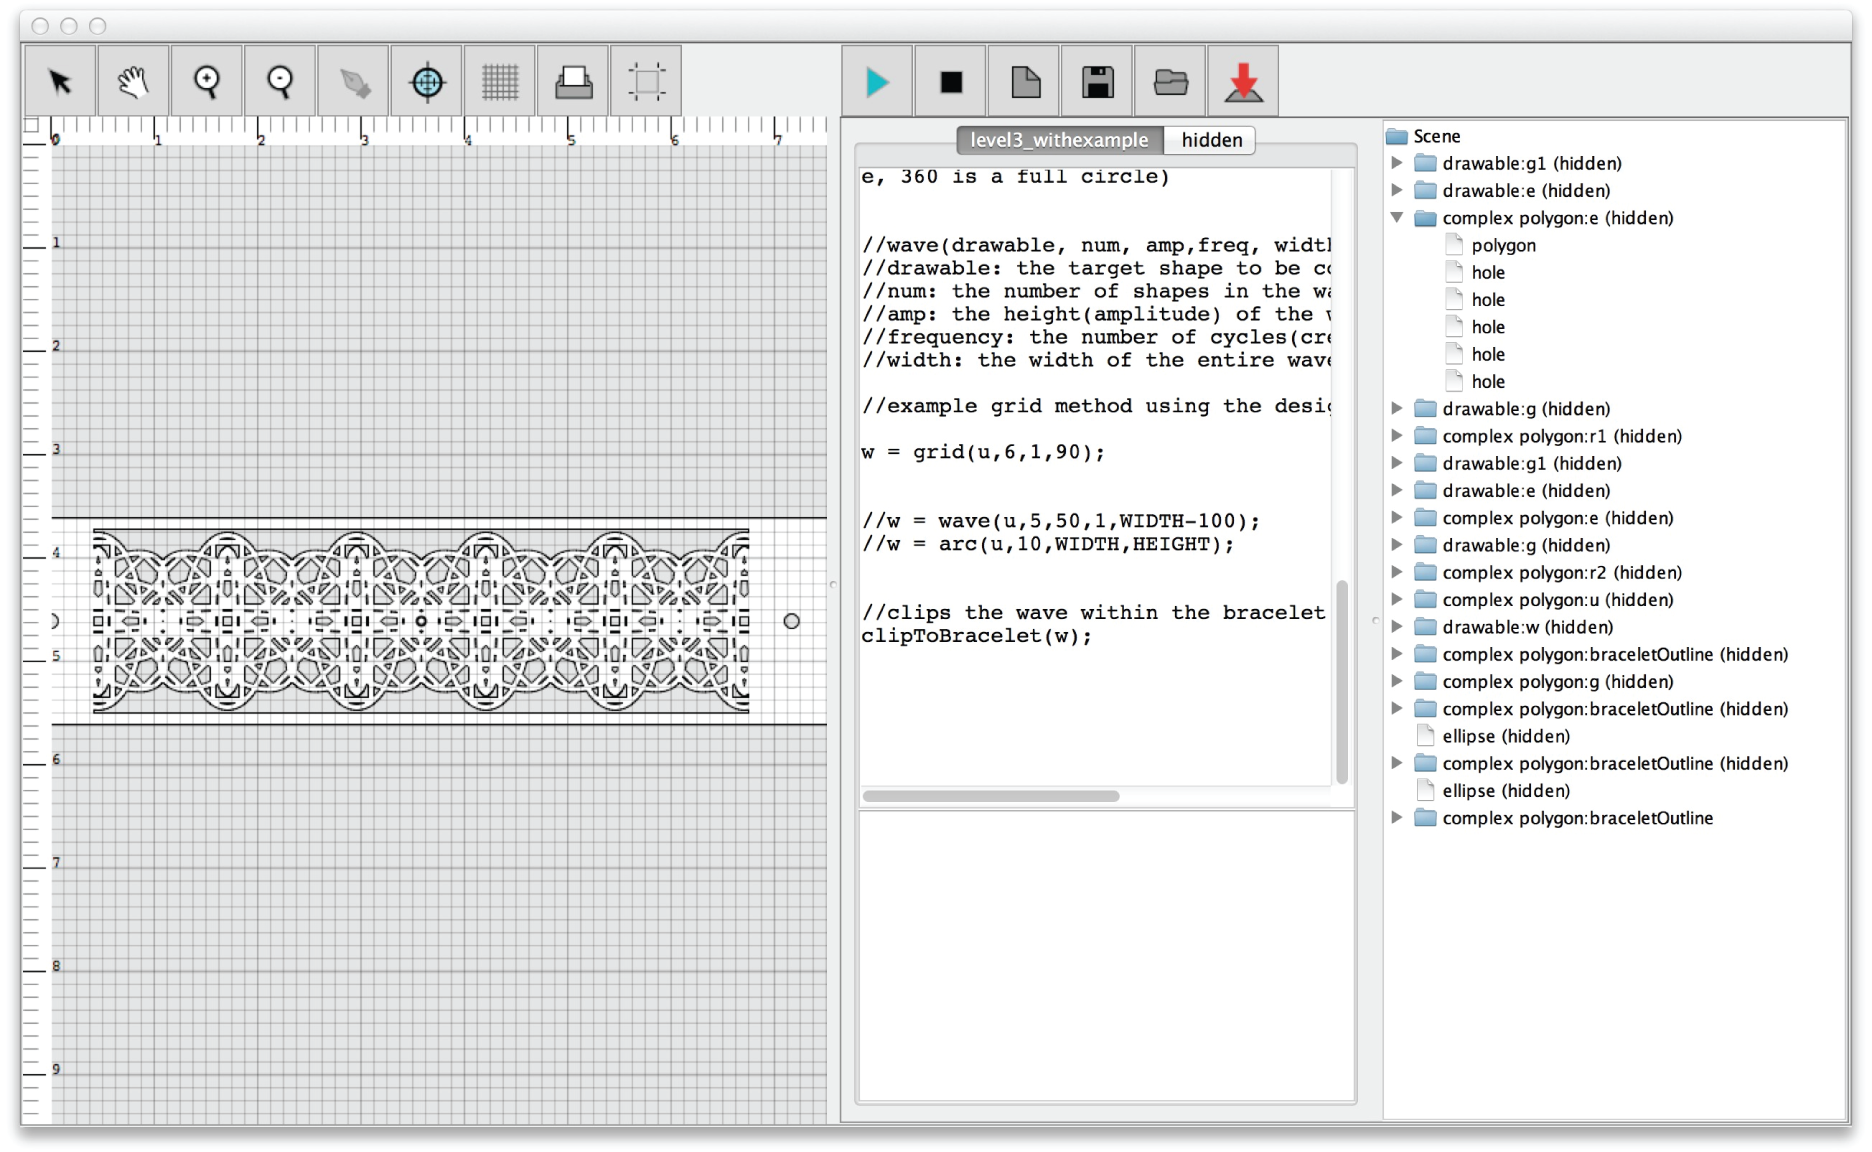
\includegraphics[width=\columnwidth]{images/declarative_view.png}
\caption{DressCode with declarative view of a design}
\label{fig:declarative_view}
\end{figure}
\end{center}

Another important area of future research is in maintaining design history and assisting in design selection. A common challenge encountered by many participants in the DressCode workshops, was the process of choosing a single design for fabrication, out of numerous possibilities: 

\begin{quotation}
\textit{``As you can see saved 10 different versions so I would save something, not a completed version of it, but as I was going a long and just do random things to it and see what happened, and if I was physically drawing it, I couldn't just do that unless I wanted to just keep erasing and re-drawing, but in this it's simple as just typing in another number and it will change, but you can always go back to what you had, so it's nice like that."}
\\Youth Participant R
\end{quotation}

As mentioned earlier, the issue of design selection is not unique to DressCode, but an inherent quality of computational design. Because algorithmic craft depends on the creation of discrete physical artifacts, design selection in algorithmic craft is a more urgent issue than in other forms of computational design. Future research could explore methods of evaluating numerous designs and in providing people with mechanisms for selection. 

Related to the issue of design selection is that of design history. Participants in all of the workshops often created designs that were later lost due to numerous changes in their code. They also often wished to merge components of two separate designs, or selectively undo some but not all of the changes to a new design. All of these challenges suggest the need for some form of version control in algorithmic craft software. If implemented correctly, version control could not only give people better control of the history of their designs, but also increase the ability to share work, and contribute to the work of others.

Finally, more research must be done in incorporating the practices and values of craft. Although craft was one of the founding components of this thesis, much of the development time was focused on writing software and learning about the properties of digital fabrication. For future research, I wish to seek the expertise of established craftspeople to gain a better understanding of craft practices and how they can be connected to computational design and digital fabrication. One possibility would be to engage in the collaborative design of a sample algorithmic crafting tool with a group of people who are experienced in a particular form of hand-craft, like garment creation or jewelry making.

\section{Conclusion}
	As computers grow in sophistication, complexity and ubiquity, it becomes possible to regard computation as a dismebodied force, outside the reach of most individuals, and incompatible with familiar forms of making. In my experience, the opposite is true. Computers offer one of the most potent forms of personal expression, by helping us to see the world in new ways. Computation does not invalidate other forms of creation, it enhances them. Algorithmic craft gives people the opportunity to experience the magic and pleasure that is possible when using programing, digital fabrication and one's hands to build something entirely new. 
	
	
	
	
	
	
	